\documentclass[document,border=0pt]{standalone}

\usepackage{tikz}
\usepackage{color}

\begin{document}
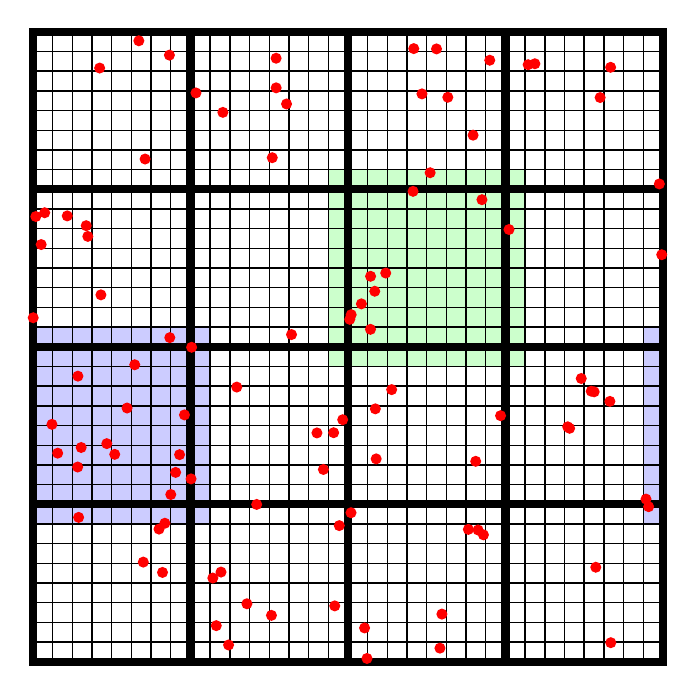
\begin{tikzpicture}

\pgfmathsetseed{1723}

\fill[green!20!white, line width=0.5] (3.75,3.75) rectangle (6.25,6.25);

\fill[blue!20!white,  line width=0.5] (0, 1.75) rectangle (2.25,4.25);
\fill[blue!20!white,  line width=0.5] (7.75, 1.75) rectangle (8,4.25);

\draw[step=0.25   ,black,line width=0.5] (0,0) grid (8,8);
\draw[step=2   ,black,line width=3] (0,0) grid (8,8);
\draw[black,line width=3] (0,0) rectangle (8,8);

\foreach \i in {1,...,100}
  \fill[red] (rnd*8cm, rnd*8cm) circle (2.0pt);

\end{tikzpicture}
\end{document}
